\documentclass{beamer}
\usetheme{Singapore}
\usepackage[utf8]{inputenc}
\usecolortheme{crane}
\usepackage{graphicx}
\usepackage{iwona}
\usepackage{standalone}
\usepackage{tikz}
\usetikzlibrary{arrows}
\usetikzlibrary{decorations.markings}
\usetikzlibrary{calc}
\usetikzlibrary{shapes,snakes}
\usepackage{amsmath}
\usepackage{amsfonts}
\usepackage{amsthm}
\usepackage{mathtools}
\usepackage{tcolorbox}
\usepackage{float}
\usepackage{bm}
\usepackage{minted}

\definecolor{lightblue}{RGB}{124,190,255}
\definecolor{darkgreen}{RGB}{24,145,0}
\definecolor{darkorange}{RGB}{220,110,0}



\beamertemplatenavigationsymbolsempty
\setbeamerfont{caption}{size=\tiny}


\title{The Ciw Python Library}
\author{Geraint Ian Palmer\\ \textcolor{darkorange}{@GeraintPalmer} $\quad$ \textcolor{darkorange}{@CiwPython}}
\date{17th April 2018}
\titlegraphic{
\includegraphics[width=2.35cm]{logos/cflogo} $\quad$ 
\includegraphics[width=2.4cm]{logos/ciw_logo}}



\begin{document}

\frame{\titlepage}


\begin{frame}
\begin{figure}
    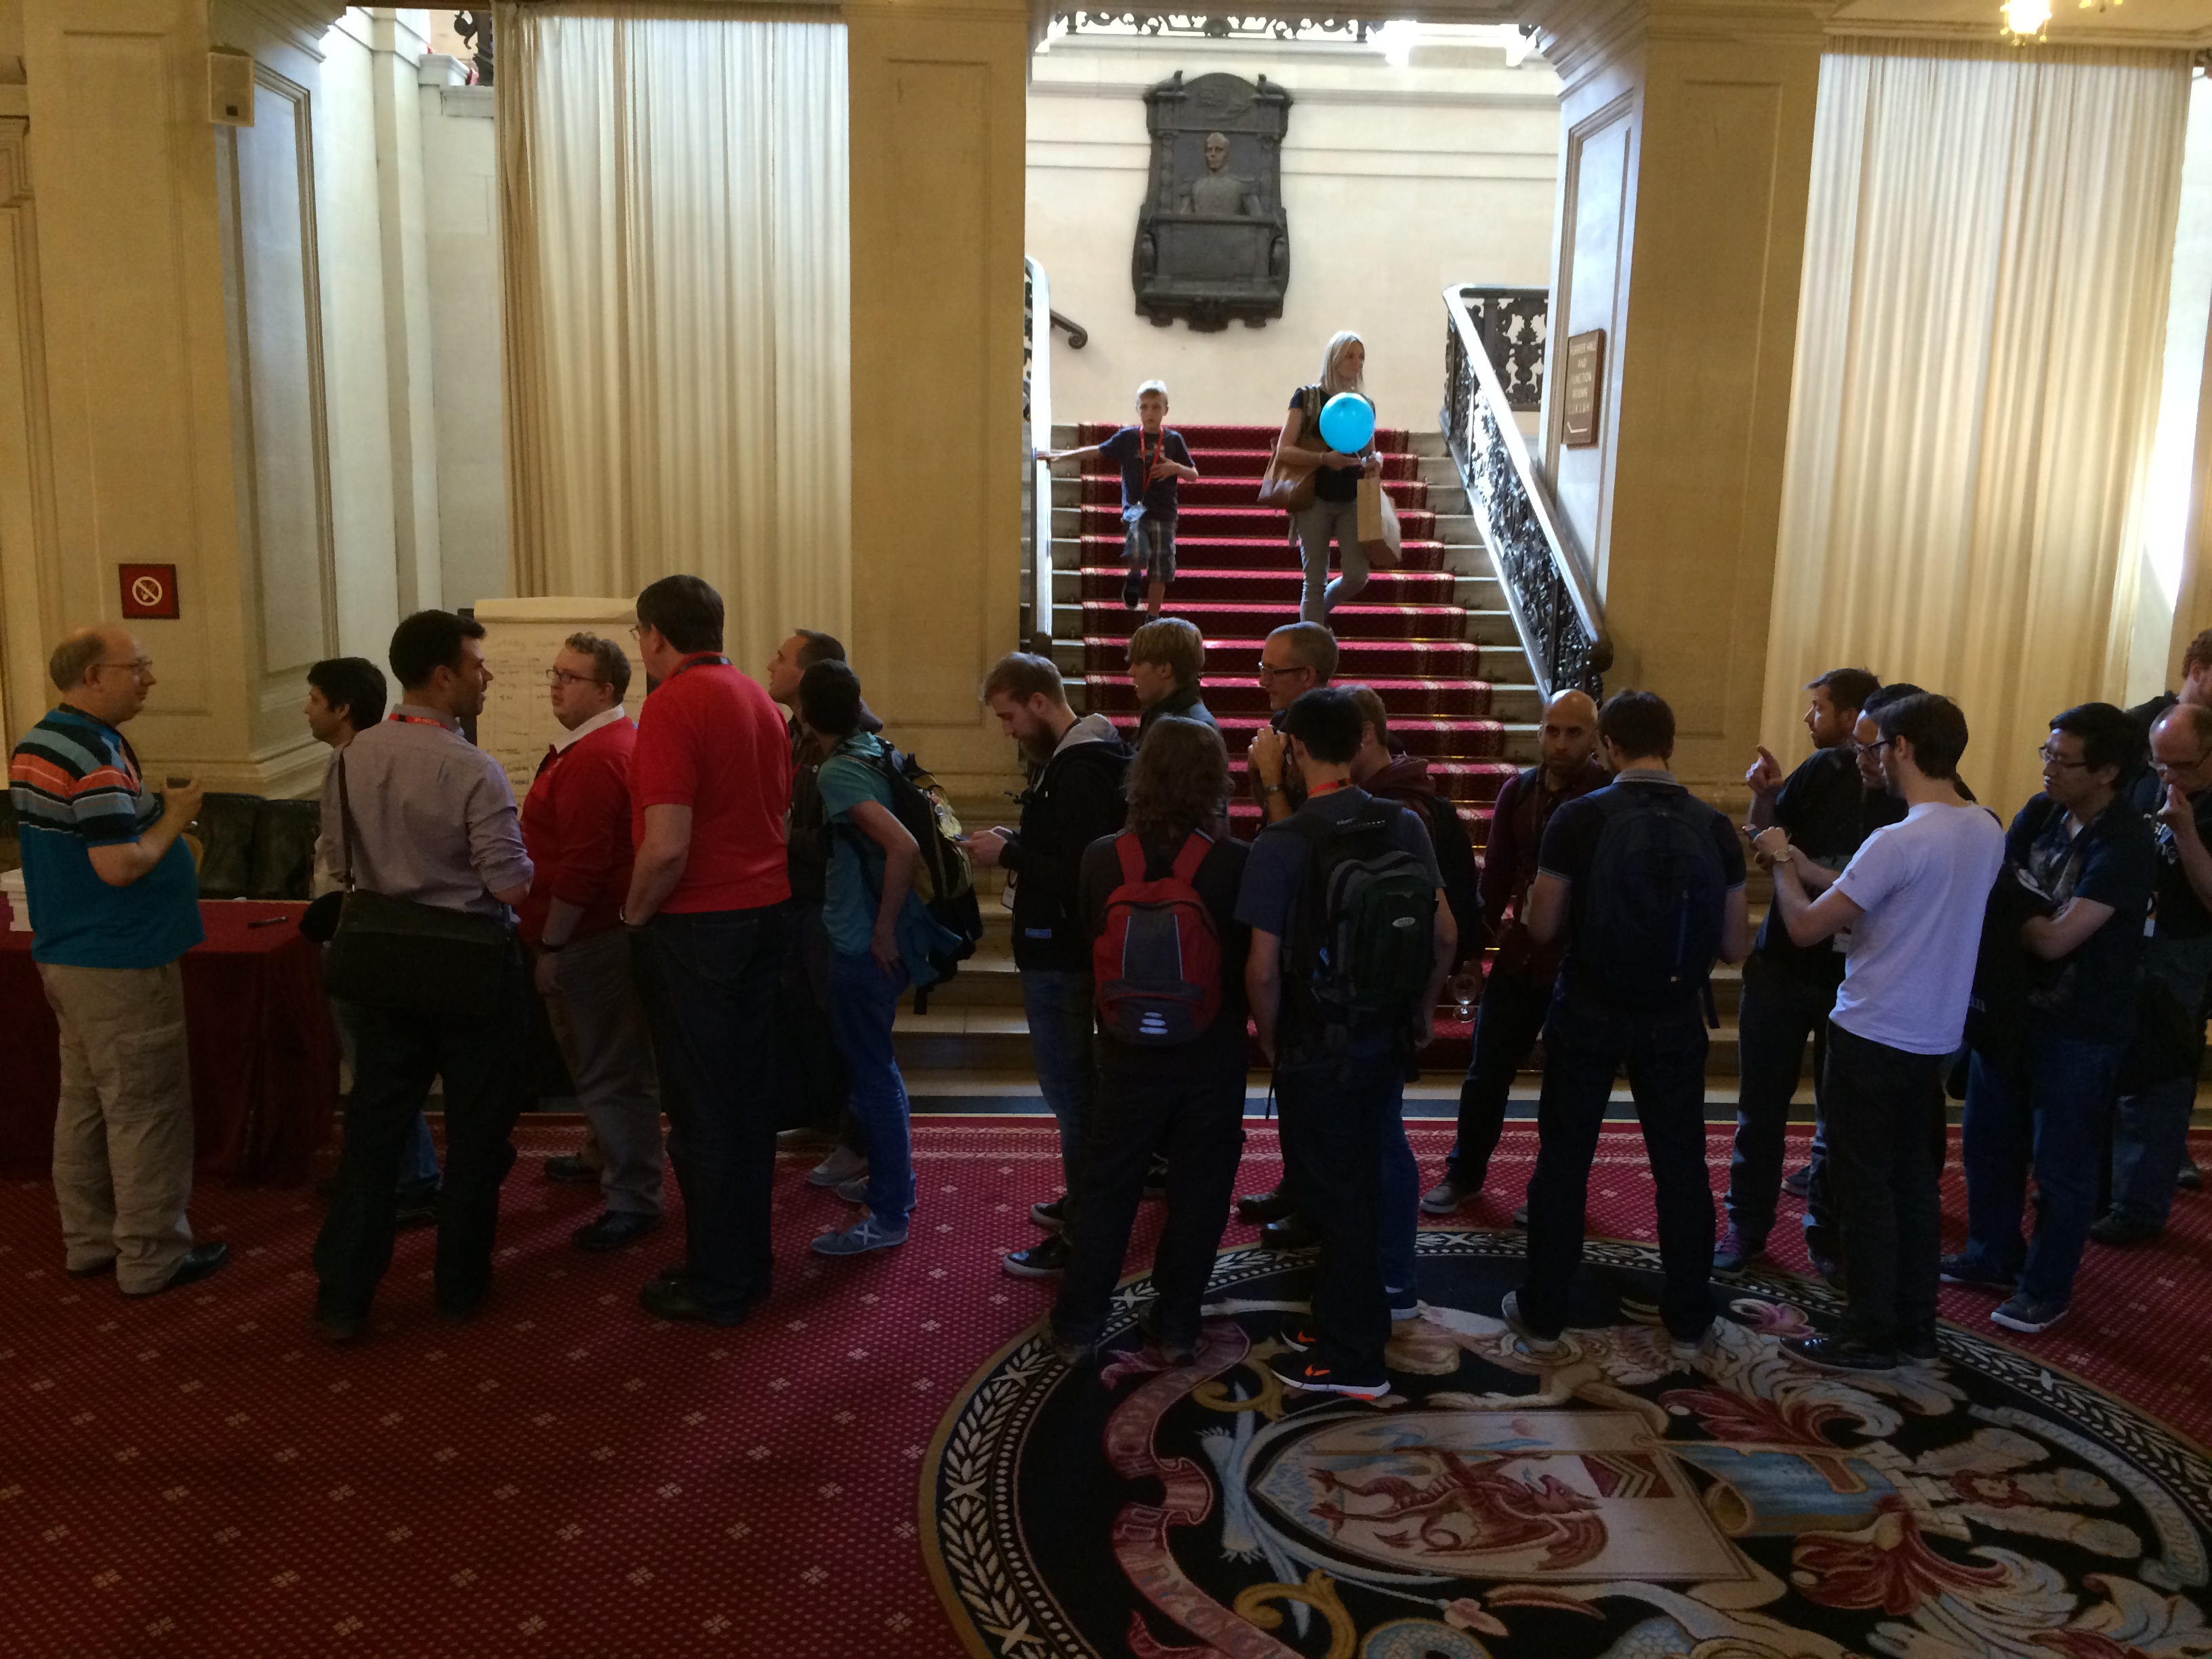
\includegraphics[width=\textwidth]{pyconqueue}
\end{figure}
\end{frame}

\begin{frame}
\begin{figure}
    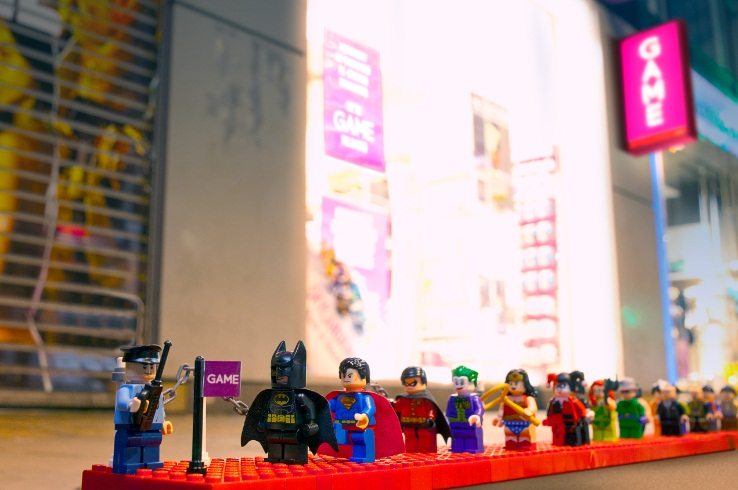
\includegraphics[width=\textwidth]{legoqueue}
\end{figure}
\end{frame}

\begin{frame}
\frametitle{What is a Queue?}
\begin{figure}
  \includestandalone[width=0.8\textwidth]{1nodeexample}
\end{figure}
\end{frame}

\begin{frame}
\frametitle{What is a Queue?}
\begin{figure}
  \includestandalone[width=0.8\textwidth]{2nodefeedbackexample}
\end{figure}
\end{frame}


\begin{frame}
\frametitle{Features}
\begin{center}
\textcolor{darkorange}{\url{http://ciw.readthedocs.io}}\\
\end{center}
\end{frame}

\begin{frame}
\frametitle{Distributions}
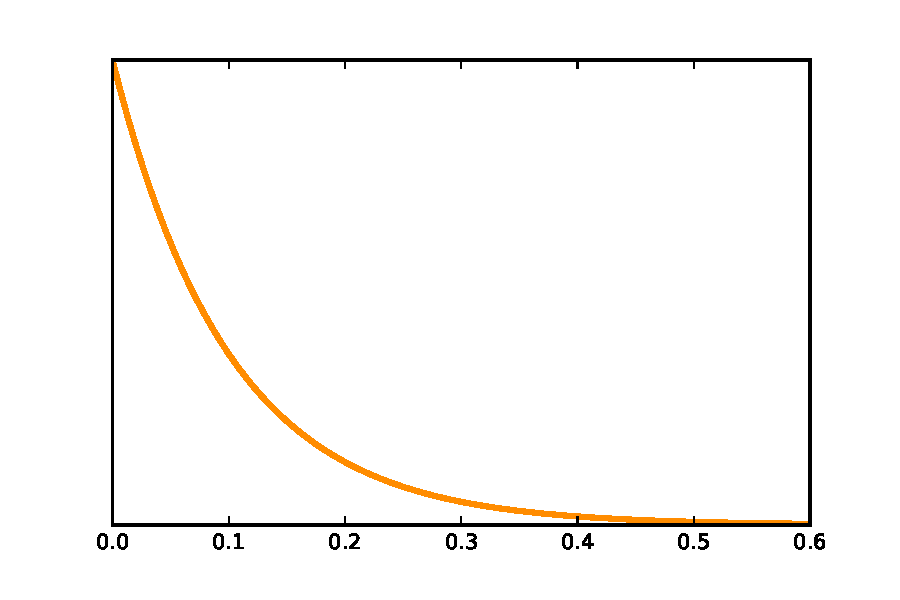
\includegraphics[width=0.48\textwidth]{expondist.pdf}
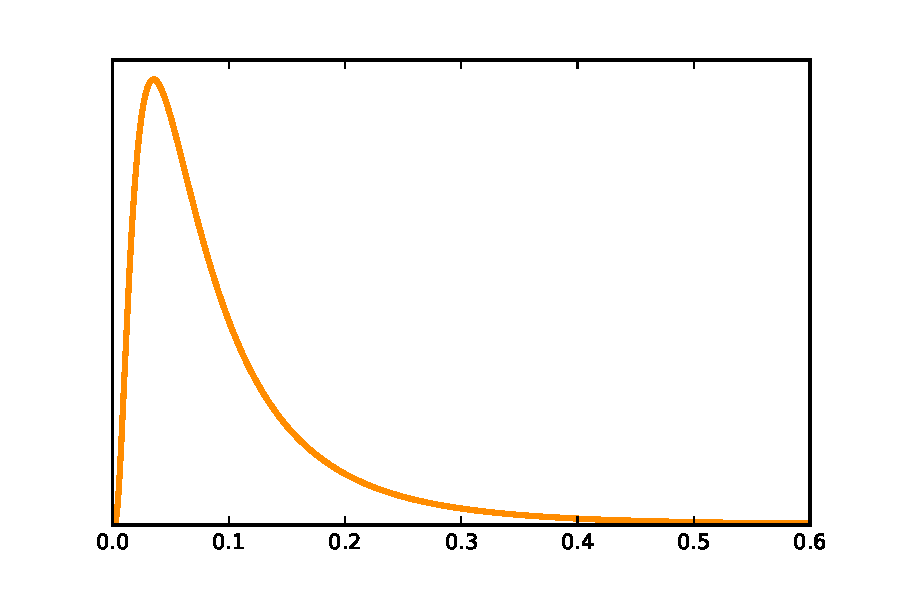
\includegraphics[width=0.48\textwidth]{lognormdist.pdf}\\
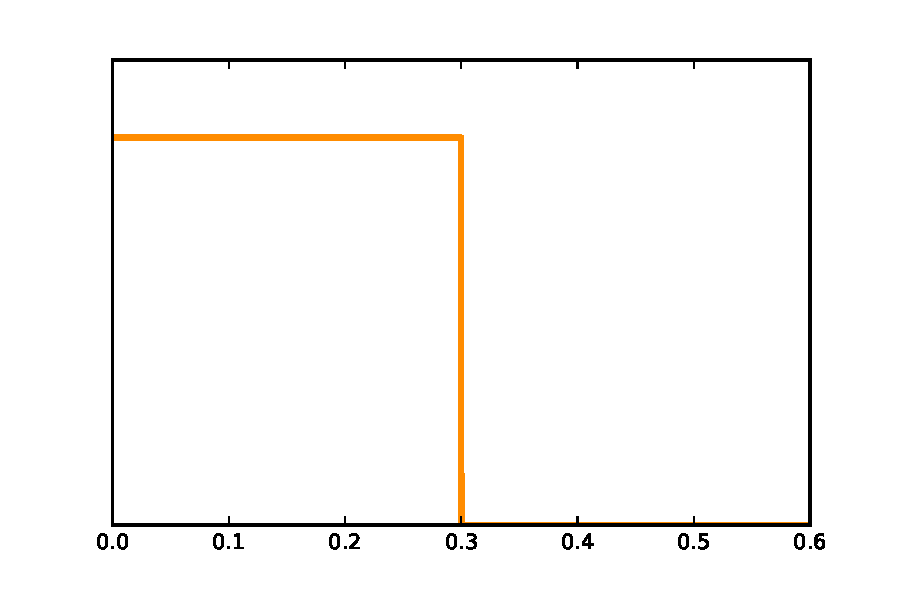
\includegraphics[width=0.48\textwidth]{uniformdist.pdf}
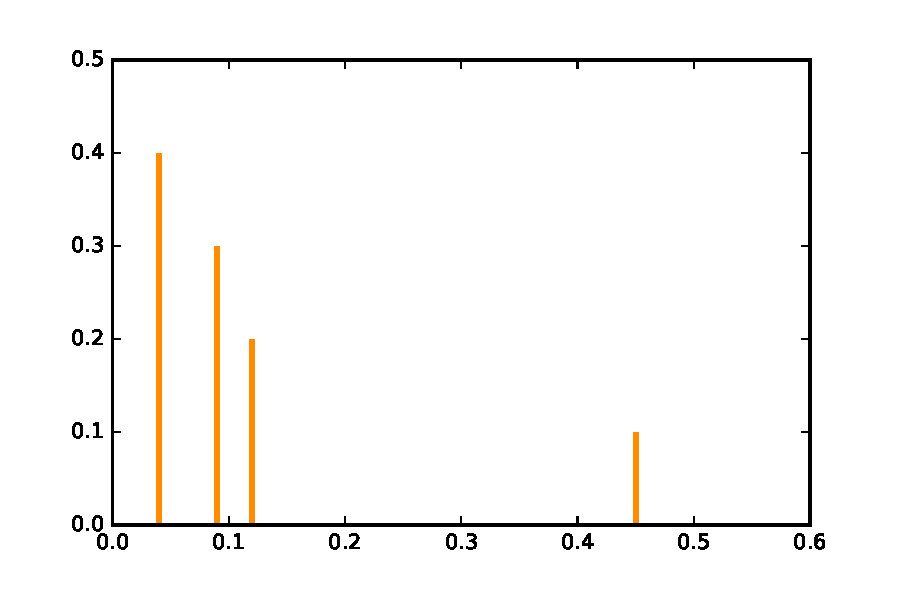
\includegraphics[width=0.48\textwidth]{custom.pdf}
\end{frame}

\begin{frame}
\frametitle{Priority Queues}
\begin{figure}
  \includestandalone[width=0.8\textwidth]{priorityexample}
\end{figure}
\end{frame}

\begin{frame}
\frametitle{Baulking}
\begin{figure}
  \includestandalone[width=\textwidth]{baulkingexample}
\end{figure}
\begin{equation*}
P(\text{baulk} \nonscript\; | \nonscript\; x \text{ in queue}) = b(x)
\end{equation*}
\end{frame}

\begin{frame}
\begin{equation*}
b(x) = \left\{ \begin{array}{cc} \frac{x}{20} & \text{ if } x \leq 2\\[4pt] \frac{x}{x+3} & \text{ if } 2 < x \leq 10\\[4pt] 1 & \text{ otherwise}\end{array} \right.
\end{equation*}\\
\begin{center}
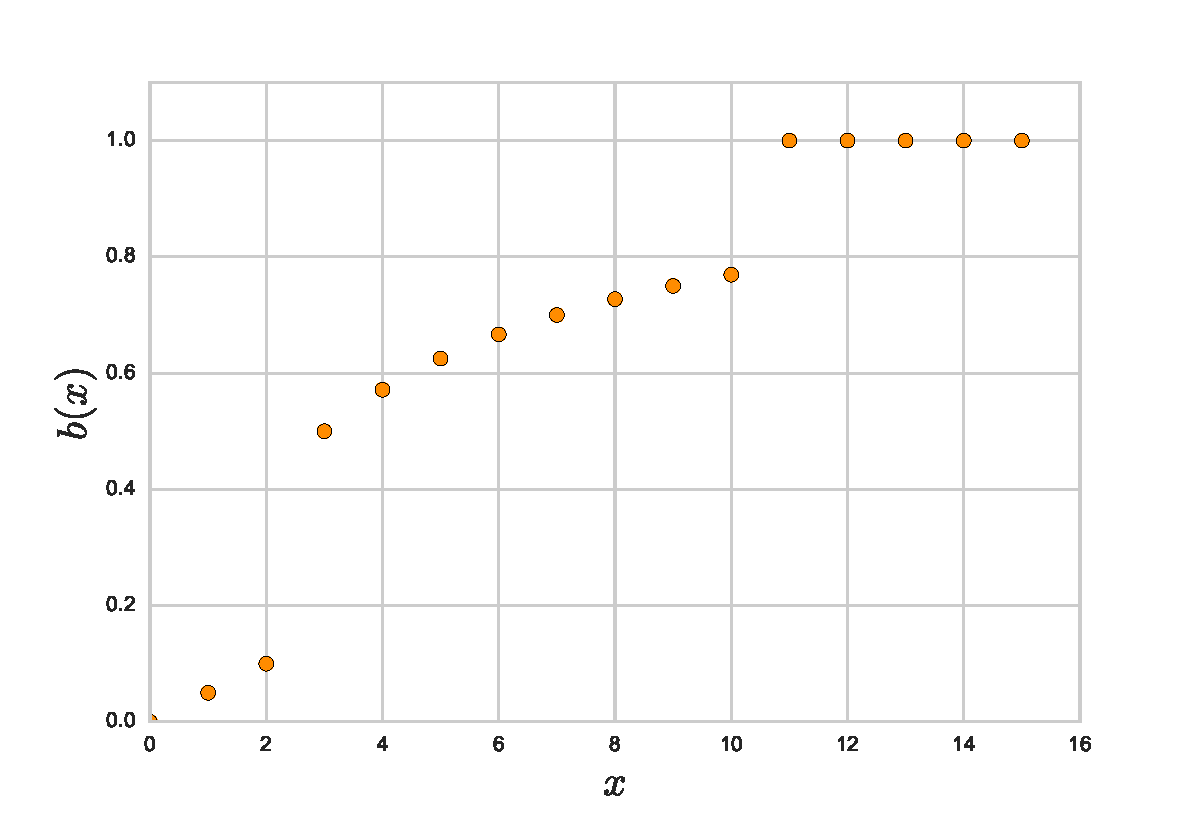
\includegraphics[width=0.72\textwidth]{baulkfunc.pdf}
\end{center}
\end{frame}

\begin{frame}
\frametitle{Server Schedules}
\includestandalone[width=\textwidth]{scheduledexample}
\end{frame}

\begin{frame}
\includestandalone[width=\textwidth]{scheduleoverlaps}
\end{frame}


\begin{frame}
\frametitle{Academic Uses}
\vfill
\begin{block}{Theoretical Work}
Investigating deadlock in queueing networks.\\
(Geraint Palmer, Prof. Paul Harper, Dr. Vincent Knight)
\end{block}
\vfill
\begin{block}{Practical Work}
Modelling an ophthalmology clinic to strategise scheduling.\\
(Lieke H\"{o}lscher, Dr. Jennifer Morgan)
\end{block}
\vfill
\begin{block}{Practical Work}
Modelling Stay Well Plans in Gwent.\\
(Geraint Palmer, Cathy Brooks, Prof. Paul Harper, Dr. Vincent Knight)
\end{block}
\vfill
\end{frame}

\begin{frame}
\frametitle{Investigating Deadlock}
\begin{figure}
    \includestandalone[width=\textwidth]{deadlock_digraph}
\end{figure}
\end{frame}

\begin{frame}
\begin{figure}
    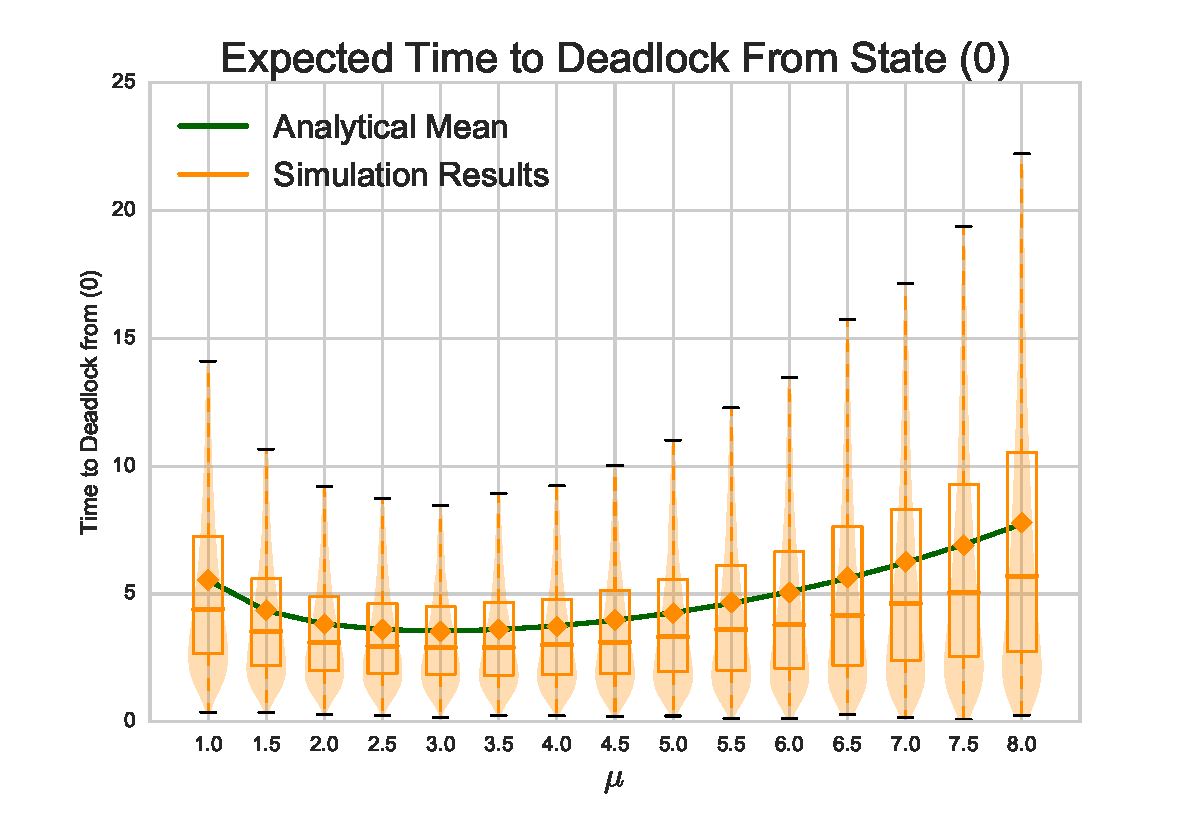
\includegraphics[width=0.95\textwidth]{varymu_1Nms}
\end{figure}
\end{frame}

\begin{frame}
\begin{center}
  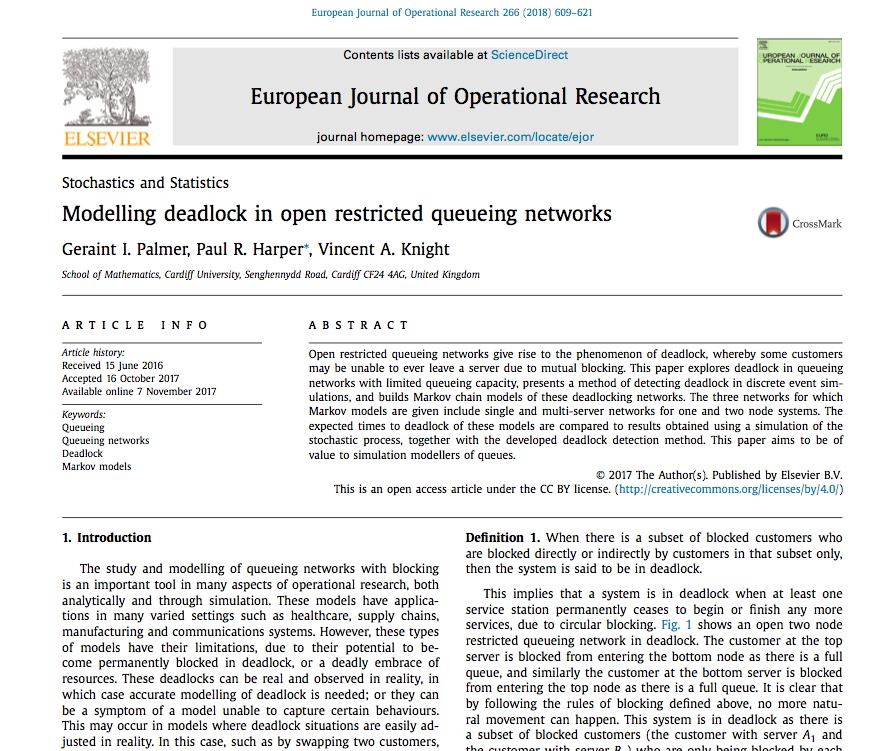
\includegraphics[width=0.65\textwidth]{deadlockpaper}
\end{center}
\small{\textcolor{darkorange}{2018: \textbf{Modelling Deadlock in Open Restricted Queueing Networks}, \textit{Palmer GI, Harper PR, Knight VA.} European Journal of Operational Research.}}
\end{frame}

\begin{frame}
\frametitle{Modelling Ophthalmology Clinic}
\begin{figure}
    \includestandalone[width=0.9\textwidth]{ophthalmology}
\end{figure}
\end{frame}

\begin{frame}
\frametitle{Modelling Stay Well Plans in Gwent}
\begin{center}
  \includestandalone[width=0.7\textwidth]{ophcn_map}
\end{center}
\end{frame}

\begin{frame}
\begin{center}
  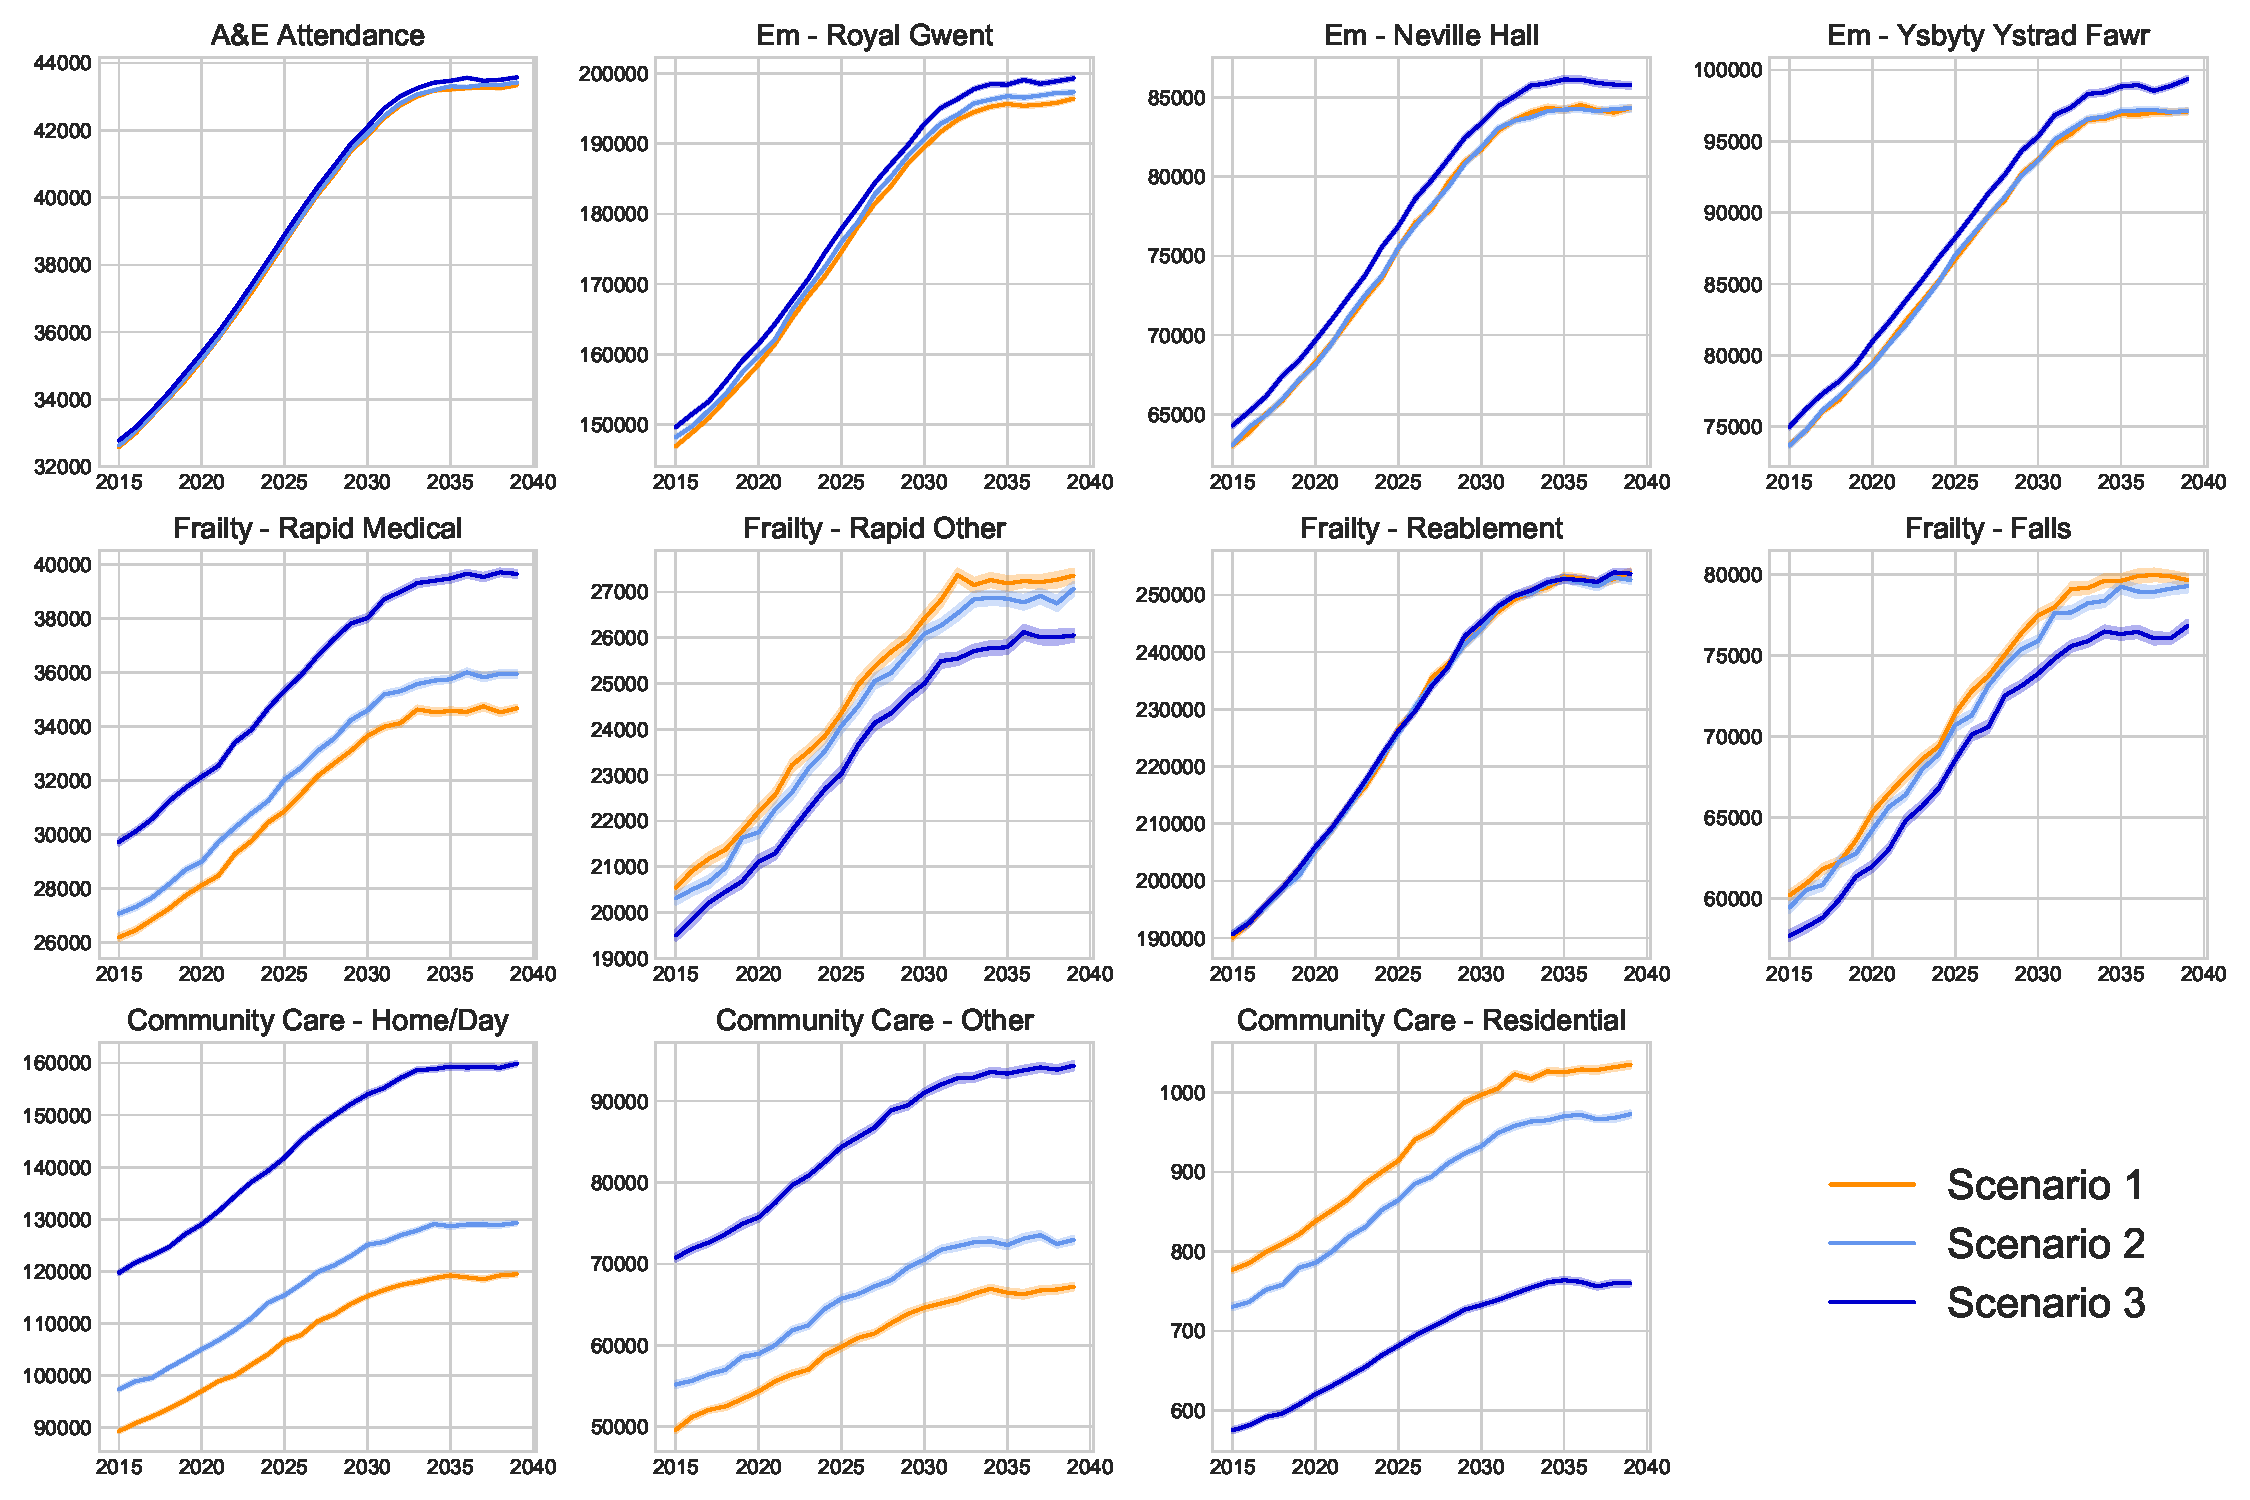
\includegraphics[width=\textwidth]{results_years}
\end{center}
\end{frame}

\begin{frame}
\frametitle{Paper on Ciw Itself}
\textcolor{darkorange}{2018: \textbf{Ciw: An open source discrete event simulation library}, \textit{Palmer GI, Knight VA, Harper PR, Hawa, AL.} (Under review at the Journal of Simulation.)}
\vfill
\begin{center}
\url{https://arxiv.org/abs/1710.03561}
\end{center}
\end{frame}

\begin{frame}[plain]
\begin{figure}
    
\includegraphics[width=\textwidth]{alllogos}
\end{figure}
\end{frame}

\begin{frame}
\frametitle{Thank you!}
\begin{center}
\textcolor{darkorange}{@GeraintPalmer}\\
\textcolor{darkorange}{@CiwPython}\\
\textcolor{darkorange}{\url{http://ciw.readthedocs.io}}\\
\textcolor{darkorange}{\url{https://github.com/CiwPython/Ciw}}\\
\vfill

\includegraphics[width=0.3\textwidth]{logos/ciw_logo.pdf}
\end{center}
\end{frame}

\end{document}